\begin{titlepage}
\begin{center}
% Upper part of the page. The '~' is needed because \\
% only works if a paragraph has started.


% Title
\HRule \\[0.4cm]
{ \huge \bfseries Einführung in die Datenanalyse mit R (700104)}\\[0.4cm]
{\Large Kursskript}

\HRule \\[1.5cm]

\begin{minipage}{0.35\textwidth}
\begin{flushleft}

\includegraphics[width=3cm,height=3cm]{misc/fig/logo_wildtierw1.png}
~\\[0.4cm]
Dr. Johannes \textsc{Signer} \\
Abteilung Wildtierwissenschaften \\
Büsgenweg 3 \\
37077 Göttingen \\[0.5cm]
\vfill
\texttt{jsigner@uni-goettingen.de}
\end{flushleft}
\end{minipage}
\hfill
\begin{minipage}{0.60\textwidth}
\begin{flushright}

\includegraphics[width=3cm,height=3cm]{misc/fig/logo_felap.png}
~\\[0.4cm]
Dr. Kai \textsc{Husmann} \\
Abteilung Forstökonomie und nachhaltige Landnutzungsplanung \\
Büsgenweg 1 \\
37077 Göttingen \\[0.5cm]
\vfill
\texttt{kai.husmann@uni-goettingen.de}
\end{flushright}
\end{minipage}


\vfill

\includegraphics[width=10cm,height=8cm]{misc/fig/logo-uni-neu.png}
~\\[0.4cm]

Fakultät für Forstwissenschaften und Waldökologie \\
Georg-August-Universität Göttingen \\[1.2cm]

\includegraphics{misc/fig/logo_cc.png}
\vfill

% Bottom of the page
\hRule ~\\[0.5cm]
{\large Wintersemester 2023/2024}\\


\end{center}
\newpage
\vspace*{\fill}
Dieses Werk ist lizenziert unter einer \href{https://creativecommons.org/licenses/by-nc-sa/4.0/}{Creative Commons Namensnennung - Nicht-kommerziell - Weitergabe unter gleichen Bedingungen 4.0 International Lizenz}. \\[1cm]
Zitiervorschlag: \\
Signer, J. und Husmann, K. (\the\year{}) Skript zur Vorlesung Einführung in die Datenanalyse mit R, Georg-August-Universität Göttingen.
~\\[1cm]
Letzte Aktualisierung: \today

\newpage

{\bf Vorwort und Danksagung} \\[0.5cm]

Lernziel des Kurses ist die Einführung in die Arbeit, Visualisierung und Analyse von (forstlichen) Datensätzen
mit dem Statistikprogramm \textit{R}. Der Schwerpunkt liegt dabei auf der Datenverarbeitung. Statistische Methoden werden nur an wenigen Stellen exemplarisch angewendet. Ein typisches Data Science Projekt besteht laut Wickham et al. (https://r4ds.hadley.nz/) aus 4 Stufen.

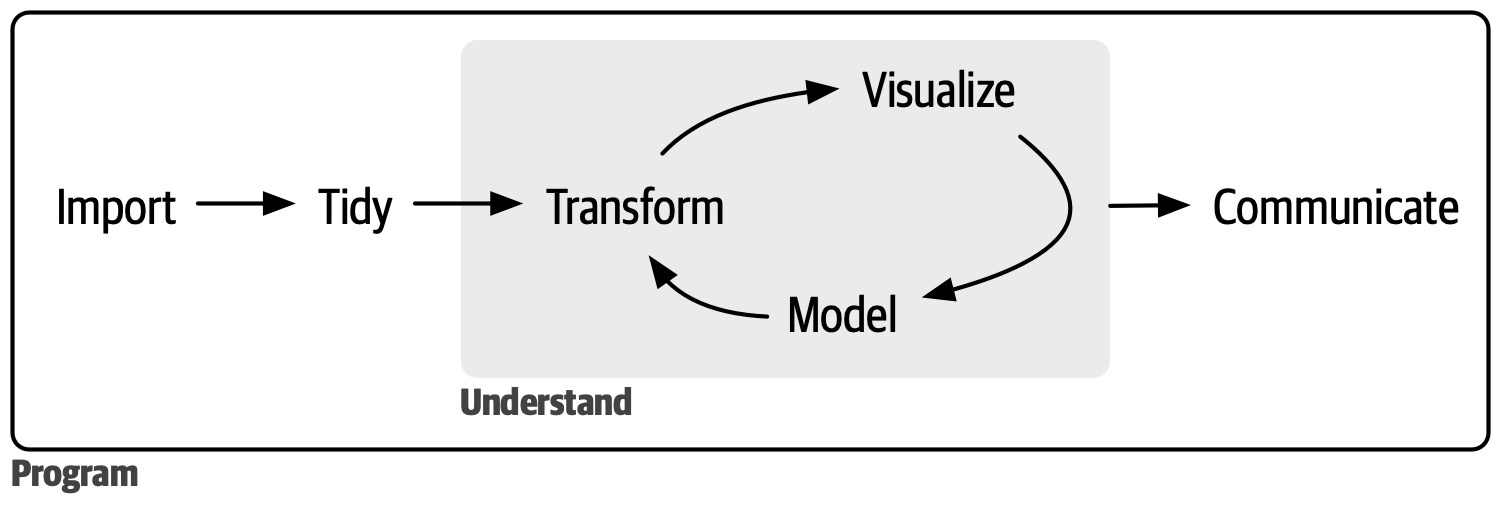
\includegraphics{img/data_science_steps.png}

Wir werden uns in diesem Kurs insbesondere mit den ersten beiden Stufen \textit{Import} und \textit{Tidy} beschäftigen und uns im Schritt \textit{Understand} nur mit sehr einfachen \textit{Models} befassen.

Weitere Materialien als dieses Kursskript und die Übungsaufgaben (StudIP) werden nicht benötigt. Die gelöste Übungsaufgaben dieses Skriptes werden Ihnen über StudIP zugänglich gemacht. Dort werden auch ggf. Ankündigungen bekanntgegeben. Um die Credits für den Kurs zu erhalten, müssen Sie am Ende des Kurses eine mündliche Prüfung ablegen. Für die Prüfung werden Sie zwei zufällig gezogene Prüfungsfragen aus dem Dokument "Übungen: Einführung in die Datenanalyse mit R" bearbeiten und vortellen.  Nach einer 15-minütigen Vorbereitungszeit beträgt die Prüfungszeit weitere 15 Minuten. In der Prüfungszeit präsentieren Sie zunächst Ihre Lösung und beantworten anschließend vertiefende Fragen zu Ihrer Lösung und daraufhin auch zum gesamten Lehrinhalt des Kurses.

Dieses Vorlesungsskript ist ein R Markdown-Dokument, das mit R und RStudio erstellt wurde. Das Dokument besteht aus Fließtext, R Code und den entsprechenden Code-Ergebnissen. Die grau hinterlegten Codepassagen sind kurze R-Skripte. Falls das Skript eine Konsolenausgabe erzeugt, ist diese direkt mit "\#\#" markiert (diese Begriffe werden in Kapitel 1.2 näher erläutert).

Dank für Anmerkungen gilt Markus Benesch, Sofie Biberacher und Josephine Trisl.
Teile des Unterkapitels zu Schleifen und Kontrollstrukturen sind an das R Skript des Kurses Computergestützte Datananalyse von Robert Nuske, Nikolas von Lüpke und Joachim Saborowski angelehnt. Des Weiteren wurden Beispiele aus dem frei Verfügbaren Dokument \textit{R for Data Science} (https://r4ds.hadley.nz/intro.html) entnommen.
\end{titlepage}

